\documentclass[a4paper,11pt,twoside]{article}
%\documentclass[a4paper,11pt,twoside,se]{article}

\usepackage{UmUStudentReport}
\usepackage{verbatim}   % Multi-line comments using \begin{comment}
\usepackage{courier}    % Nicer fonts are used. (not necessary)
\usepackage{pslatex}    % Also nicer fonts. (not necessary)
\usepackage[pdftex]{graphicx}   % allows including pdf figures
\usepackage{listings}
\usepackage{pgf-umlcd}
%\usepackage{lmodern}   % Optional fonts. (not necessary)
%\usepackage{tabularx}
%\usepackage{microtype} % Provides some typographic improvements over default settings
%\usepackage{placeins}  % For aligning images with \FloatBarrier
%\usepackage{booktabs}  % For nice-looking tables
%\usepackage{titlesec}  % More granular control of sections.

% DOCUMENT INFO
% =============
\department{Department of Computing Science}
\coursename{System Level Programming 7.5 p}
\coursecode{5DV088}
\title{Minimal Shell - MISH}
\author{Lorenz Gerber ({\tt{dv15lgr@cs.umu.se}} {\tt{lozger03@student.umu.se}})}
\date{2016-10-07}
%\revisiondate{2016-01-18}
\instructor{Mikael Ränner / Filip Åberg / Jonathan Westin / Mattias Åsander}


% DOCUMENT SETTINGS
% =================
\bibliographystyle{plain}
%\bibliographystyle{ieee}
\pagestyle{fancy}
\raggedbottom
\setcounter{secnumdepth}{2}
\setcounter{tocdepth}{2}
%\graphicspath{{images/}}   %Path for images

\usepackage{float}
\floatstyle{ruled}
\newfloat{listing}{thp}{lop}
\floatname{listing}{Listing}



% DEFINES
% =======
%\newcommand{\mycommand}{<latex code>}

% DOCUMENT
% ========
\begin{document}
\lstset{language=C}
\maketitle
\thispagestyle{empty}
\newpage
\tableofcontents
\thispagestyle{empty}
\newpage

\clearpage
\pagenumbering{arabic}

\section{Problem Description} 
The aim of this laboration was to develop a minimal unix shell. The shell had to implement input and output stream redirection, stream piping between commands and two internal commands, `cd' and `echo'. The main techniques to be used for implementing the shell were `pipes', `forking' and execution of programs by the `exec' function family. Further, the interrupt signal (SIGINT) had to be reassigned to a function that allows to stop all child processes and then returns control back to the shell prompt. A function for parsing the shell input was provided. 

\section{Compilation and Invocation}
A makefile is provided for compiling the code: `make all'. It was tested on clang 800.0.38 (OSX 10.11.6), gcc 4.9.2 (Debian) and gcc 5.4.0 (Ubuntu). Some issues where encountered regarding functionality defined in the POSIX standard. A \#define was required in the files that contain the respective functions. Another solution would have been to compile with the -std=gnu11 flag. Makefile also provides a function for cleaning up: `make clean'.

\section{Detailed Usage Description}
`mish' does not take any command line argument. The shell can be aborted by sending EOF to the prompt (Ctrl-D). SIGINT (Ctrl-C) is ignored in the prompt main loop and assigned to a function that sends SIGINT to all child processes during execution of external commands.
As specified, two internal commands, `cd' and `echo' are available. `cd' takes as argument the path, absolut or relative,  to change to. It uses internally the `chdir' function. The `echo' takes space separated strings and redirects them to STDOUT.

\section{Algorithm Description}
Below follows a description of the function that executes external commands and takes care of piping and redirection. Here, it was chosen to implement a solution where pipes are created one by one while iterating over the commands to be piped. Another solution would have been to create all pipes in advance and then just spawn processes one by one while solving the pipe routing. The current implementation always keeps the stream end for the next command 'remembered' in the parent process. On the second last command, the iteration over commands is abondend and as the last command does not need another pipe. 


\begin{verbatim}

loop over all but the last commands 
    create a pipe
    spawn a child process

    Child process code:
        if requested 
            setup redirect
        else
            close pipe read_end
        if there is a remembered file descriptor from the last iteration 
            duplicate it to STDIN and close the remembered file descriptor
        duplicate the pipes write end to STDOUT and close the pipes write end
        run command

    Parent process code:
        if there is a remembered file descriptor from the last iteration,
            close it.
        remember the the read end of the pipe 
        close the pipes write end

spawn a child process for last command

Child process code:
    if there is only one command and this command has 
        to redirect input from a file
        then redirect in_file file descriptor to STDIN

    if redirect of output to a file is requested
        redirect out_file file descriptor to STDOUT

    redirect pipe read_end to STDIN

    clean up

    run command

Parent process code:
    wait for child processes to report finished
    cleaning up
\end{verbatim}


\section{System Description}
\subsection{General structure}
The general structure of the implementation is first documented by a call graph in figure \ref{fig:callgraph}. As it can be seen, a rather flat organization was chose where most commands are called directly by the main process.
\begin{figure}
\centering
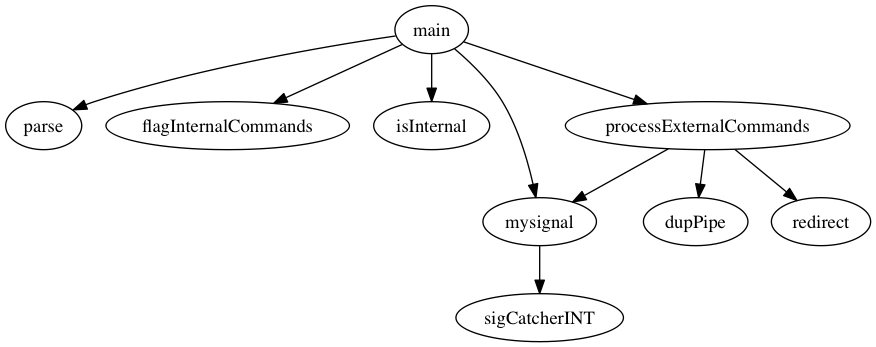
\includegraphics[width=\textwidth]{callgraph.png}
\caption{\textit{This figure shows the call graph of mish.}}
\label{fig:callgraph}
\end{figure}


\subsection{Piping and Redirection}

The basic structure for starting commands in a shell is:
\begin{enumerate}
\item open a pipe to allow inter process communication
\item fork a child processs
\item execute command in child process
\item monitor termination of the child process in the parent process
\end{enumerate}

Below follows a more detailed account for the chosen implementation of the piping and redirection functionality. Figure \ref{fig:pipes} exemplifies the sequence of commands for the piping setup with three commands, hence two pipes. 

\begin{figure}
\centering

\includegraphics[width=\textwidth]{pipes.png}
\caption{\textit{This figure shows the sequence of commands for the
    piping setup, here with three commands, hence two pipes.}}
\label{fig:pipes}
\end{figure}

\subsection{Signal Handling}
For reliable signal handling `sigaction', was implemented as function `mySignal'so that it could be used with the same call signature as `signal'. The new signal handler function for the SIGINT signal is deployed in the beginnin of the `processExternalCommands' call. It uses a global integer array that holds the pids of all started child processes and sends SIGINT by `kill' calls to each of them.

In the prompt loop of the main program, a call to `mySignal' reassigns the SIGINT function to SIG_IGN, whic prevents the shell prompt to react on Ctrl-C from the user.  


\section{Known Limits}
Currently the number of command commands to be processed on one command line entry is set to 8. 

\section{Testing}

\subsection{Debugging}
Debugging was found to be rather difficult with the child processes. Not all versions of GDB allow switching to the child process. The default GDB version available on my home setup (Ubuntu 16.04) didn't seem to react on the setting within GDB that should allow switching to the child process. Neither did it work on a custom installed GCC/GDB setup from Homebrew on a OSX 10.11.6. Hence the obvious available solution for some insight were trace printouts to stderr. 

\subsection{Testing for closing of file descriptors}
A number of trace print statements of active file descriptors was setup to monitor whether a long chain of piped commands does not result in the increase of lowest availble file descriptors value.

\subsection{Testing for correct finishing of child processes}
The `ps' command was used to monitor the correct termination of child processes. 

\addcontentsline{toc}{section}{\refname}
\bibliography{references}

\end{document}
